
 


\begin{figure}[tb]
    \centering
    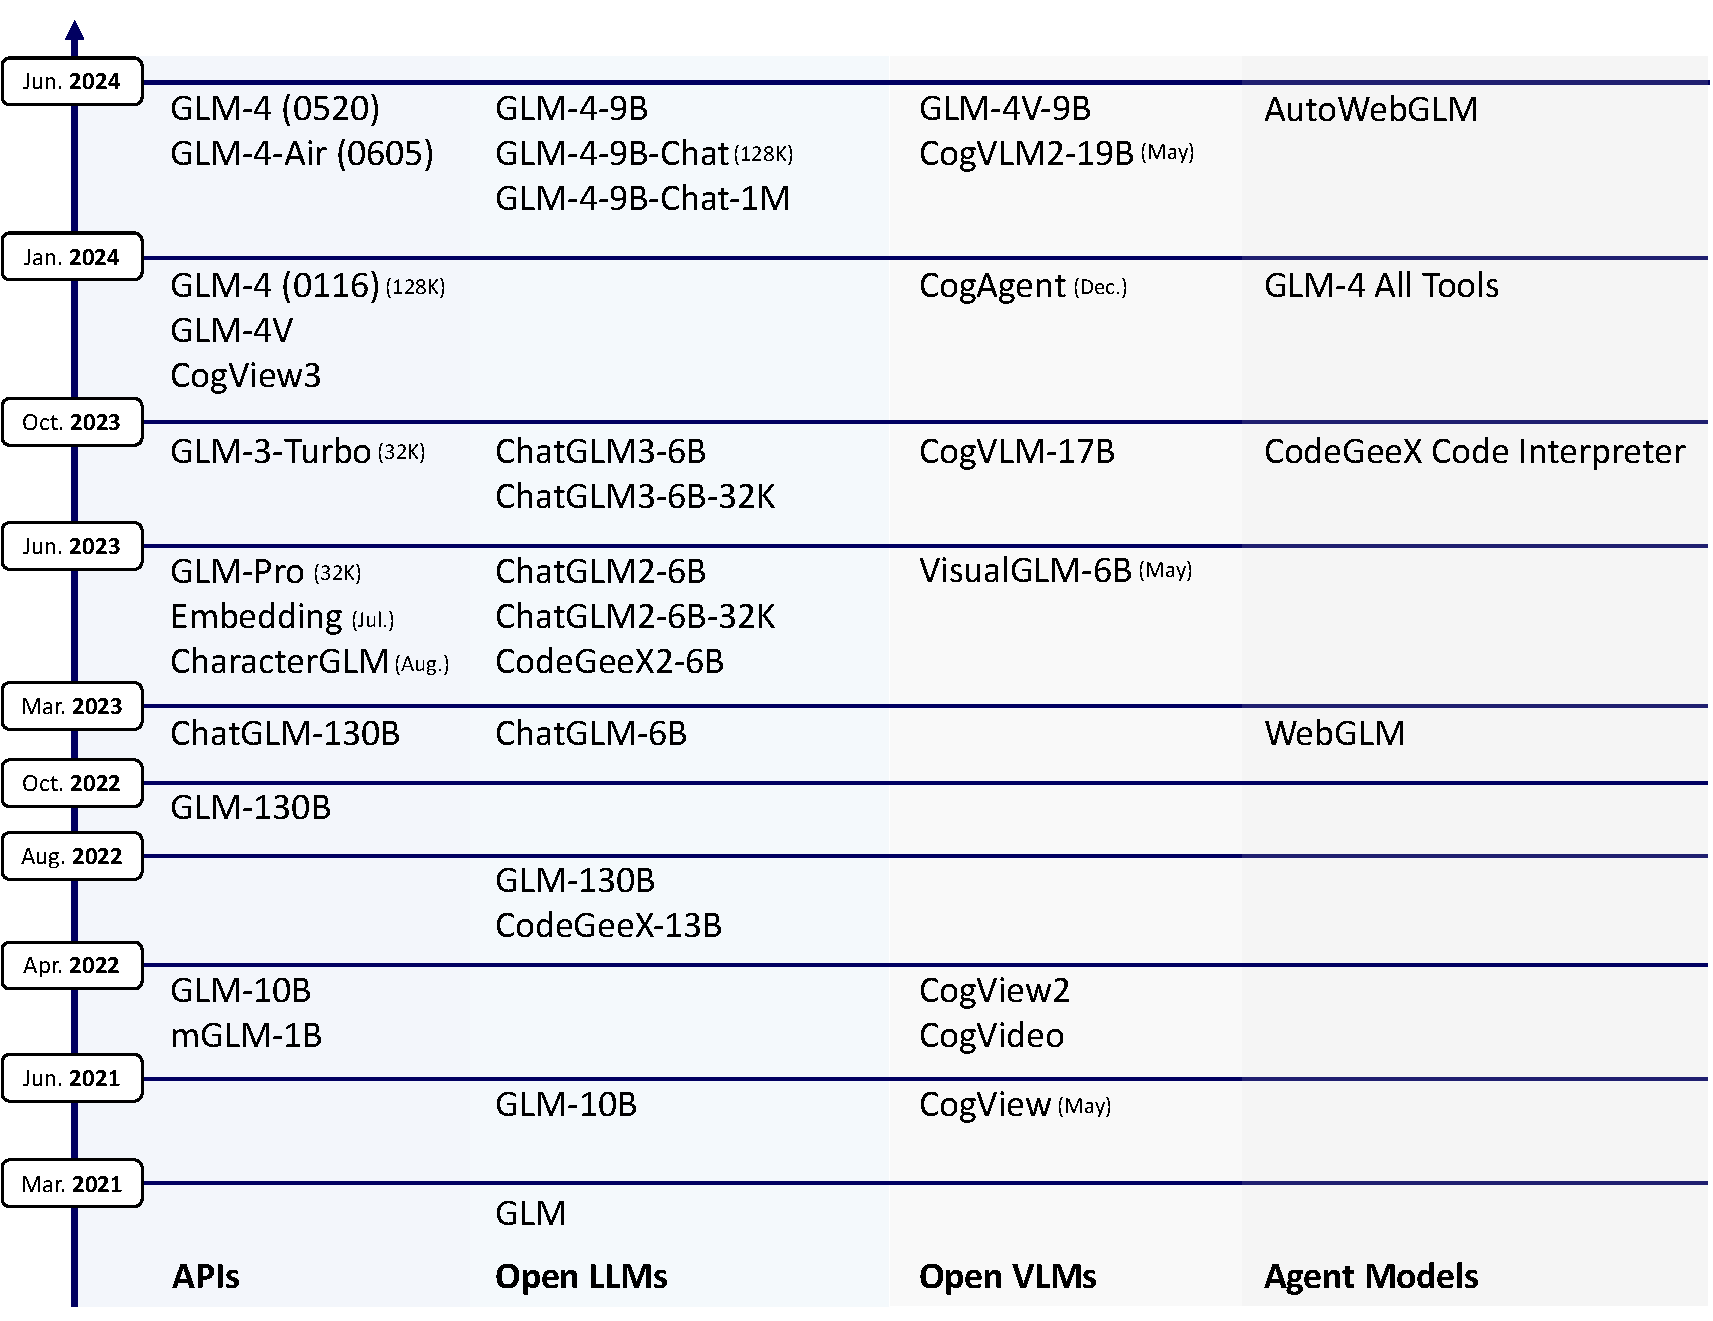
\includegraphics[width=\linewidth]{figs/glm4-history6.pdf}
    \caption{The timeline of the GLM family of language, code, vision, and agent models. The focus of this report is primarily on the language models, i.e., ChatGLM. The APIs are publicly available at \url{https://bigmodel.cn} and open models can be accessed through \url{https://github.com/THUDM}.}
    \label{fig:timeline}
\end{figure}

\section{Introduction}

ChatGPT has been phenomenal, whose capabilities was initially powered by the GPT-3.5 model~\cite{chatgpt} in November 2022 and subsequently upgraded to GPT-4~\cite{openai2023gpt} in March 2023. 
According to OpenAI, the GPT-3.5 series improved upon GPT-3 by incorporating instruction tuning, supervised fine tuning (SFT), and/or reinforcement learning from human feedback (RLHF)~\cite{ouyang2022training}. 
The original GPT-3 released in 2020~\cite{GPT3} marked a significant scale-up from GPT-1's 117 million parameters and GPT-2's 1.5 billion parameters, to 175 billion parameters. 
This scale-up enables GPT-3 with in-context learning and generalized capabilities, spurring the emergence of large language models (LLMs)~\cite{chowdhery2022palm,touvron2023llama}. 

Inspired by GPT-3, we proposed the General Language Model (GLM) architecture~\cite{du2022glm} featured with the autoregressive blank infilling objective and open-sourced the GLM-10B model in 2021 (See the GLM timeline in Figure \ref{fig:timeline}). 
Starting in late 2021, we began pre-training GLM-130B~\cite{zeng2022glm}. 
The goal was to train a 100B-scale model to match or surpass GPT-3 (davinci) while also verifying the techniques for successfully training models at this scale, along with  other efforts such as OPT-175B~\cite{zhang2022opt} and BLOOM-176B~\cite{scao2022bloom}. 
We completed the 400B-token training and evaluation of GLM-130B in July, and subsequently released the model and pre-training details~\cite{zeng2022glm} in August 2022. 
According to HELM in November 2022, GLM-130B matches GPT-3 (davinci) across various dimensions~\cite{liang2023holistic}. 


Following this, we initiated instruction tuning on GLM-130B. 
Later, ChatGPT further motivated us to align the base models with SFT and RLHF. 
We created and crafted the prompt-response pairs from scratch and performed SFT, while also starting to examine how to effectively apply RLHF. 
On March 14, 2023, the aligned model, ChatGLM-130B, went live on \url{https://chatglm.cn}. 
In addition, a smaller version, ChatGLM-6B~\cite{github:chatglm-6b}, was open-sourced at the same day, attracting significantly more attention than anticipated. 
It was designed to have 6.2 billion parameters for 1) facilitating fast iteration of pre-and post-training techniques as well as data selection, and 2) enabling local deployment on consumer-grade graphics cards using INT4 quantization. 
Since then, we have been rapidly exploring and refining our pre-training and alignment techniques, leading to the second and third generations of ChatGLM series every other three months, both of which were pre-trained entirely from the beginning. 


ChatGLM-6B was pre-trained on approximately one trillion tokens of Chinese and English corpus with a context length of 2,048 (2K), supplemented mostly by SFT.
Released in June, ChatGLM2-6B was pre-trained and aligned with more and better data, leading to substantial improvements over its predecessor, including a 23\% improvement on MMLU, 571\% on GSM8K, and 60\% on BBH. 
By adopting the FlashAttention technique~\cite{dao2022flashattention}, its context length was extended to 32K. 
Additionally, the integration of Multi-Query Attention~\cite{shazeer2019fast} contributed to a 42\% increase in inference speed. 
Taking this further, our 2nd generation code model CodeGeeX2-6B was developed by pre-training on an additional 600 billion code tokens. 
It demonstrates Pass@1 improvements over the initial generation, CodeGeeX-13B~\cite{zheng2023codegeex}, with increases of 57\% in Python, 71\% in C++, 54\% in Java, 83\% in JavaScript, and 56\% in Go  as measured by HumanEval-X. 
By further realizing more diverse training datasets, more sufficient training steps, and more optimized training strategies, ChatGLM3-6B topped 42 benchmarks across semantics, mathematics, reasoning, code, and knowledge. 
Starting from this generation, ChatGLM also supports function call and code interpreter, as well as complex agent tasks~\cite{deng2023mind2web,shridhar2020alfworld,yao2022webshop}. 
In the course of these developments, we also developed models with 1.5B, 3B, 12B, 32B, 66B, and 130B parameters, allowing us to validate our observations and establish our own scaling laws. 



With all the lessons learned and experiences accumulated, we kicked off the training of GLM-4. 
The first cutoff checkpoint then underwent a multi-stage post-training process (e.g., SFT, RLHF, safety alignment) with a focus on the Chinese and English language for now. 
Subsequently, it was developed into two distinct versions: GLM-4 and GLM-4 All Tools, both supporting a 128K context length. 
Since Jan. 16, 2024, GLM-4 (0116) has been made available through the GLM-4 API at \url{https://bigmodel.cn}, and GLM-4 All Tools is accessible via the website \url{https://chatglm.cn} and mobile applications that support the creation of one's own agent---GLMs. 
The latest models are GLM-4 (0520) and GLM-4-Air (0605) with an upgrade on both pre-training and alignment. 
GLM-4-Air achieves comparable performance to GLM-4 (0116) with lower latency and inference cost. 
Evaluations of GLM-4 were performed on a variety of language benchmarks. 
These evaluations assess GLM-4's general abilities in English, instruction following in both English and Chinese, and alignment, long-context, and agent capacities in Chinese.  

\begin{figure}[tb]
    \centering
    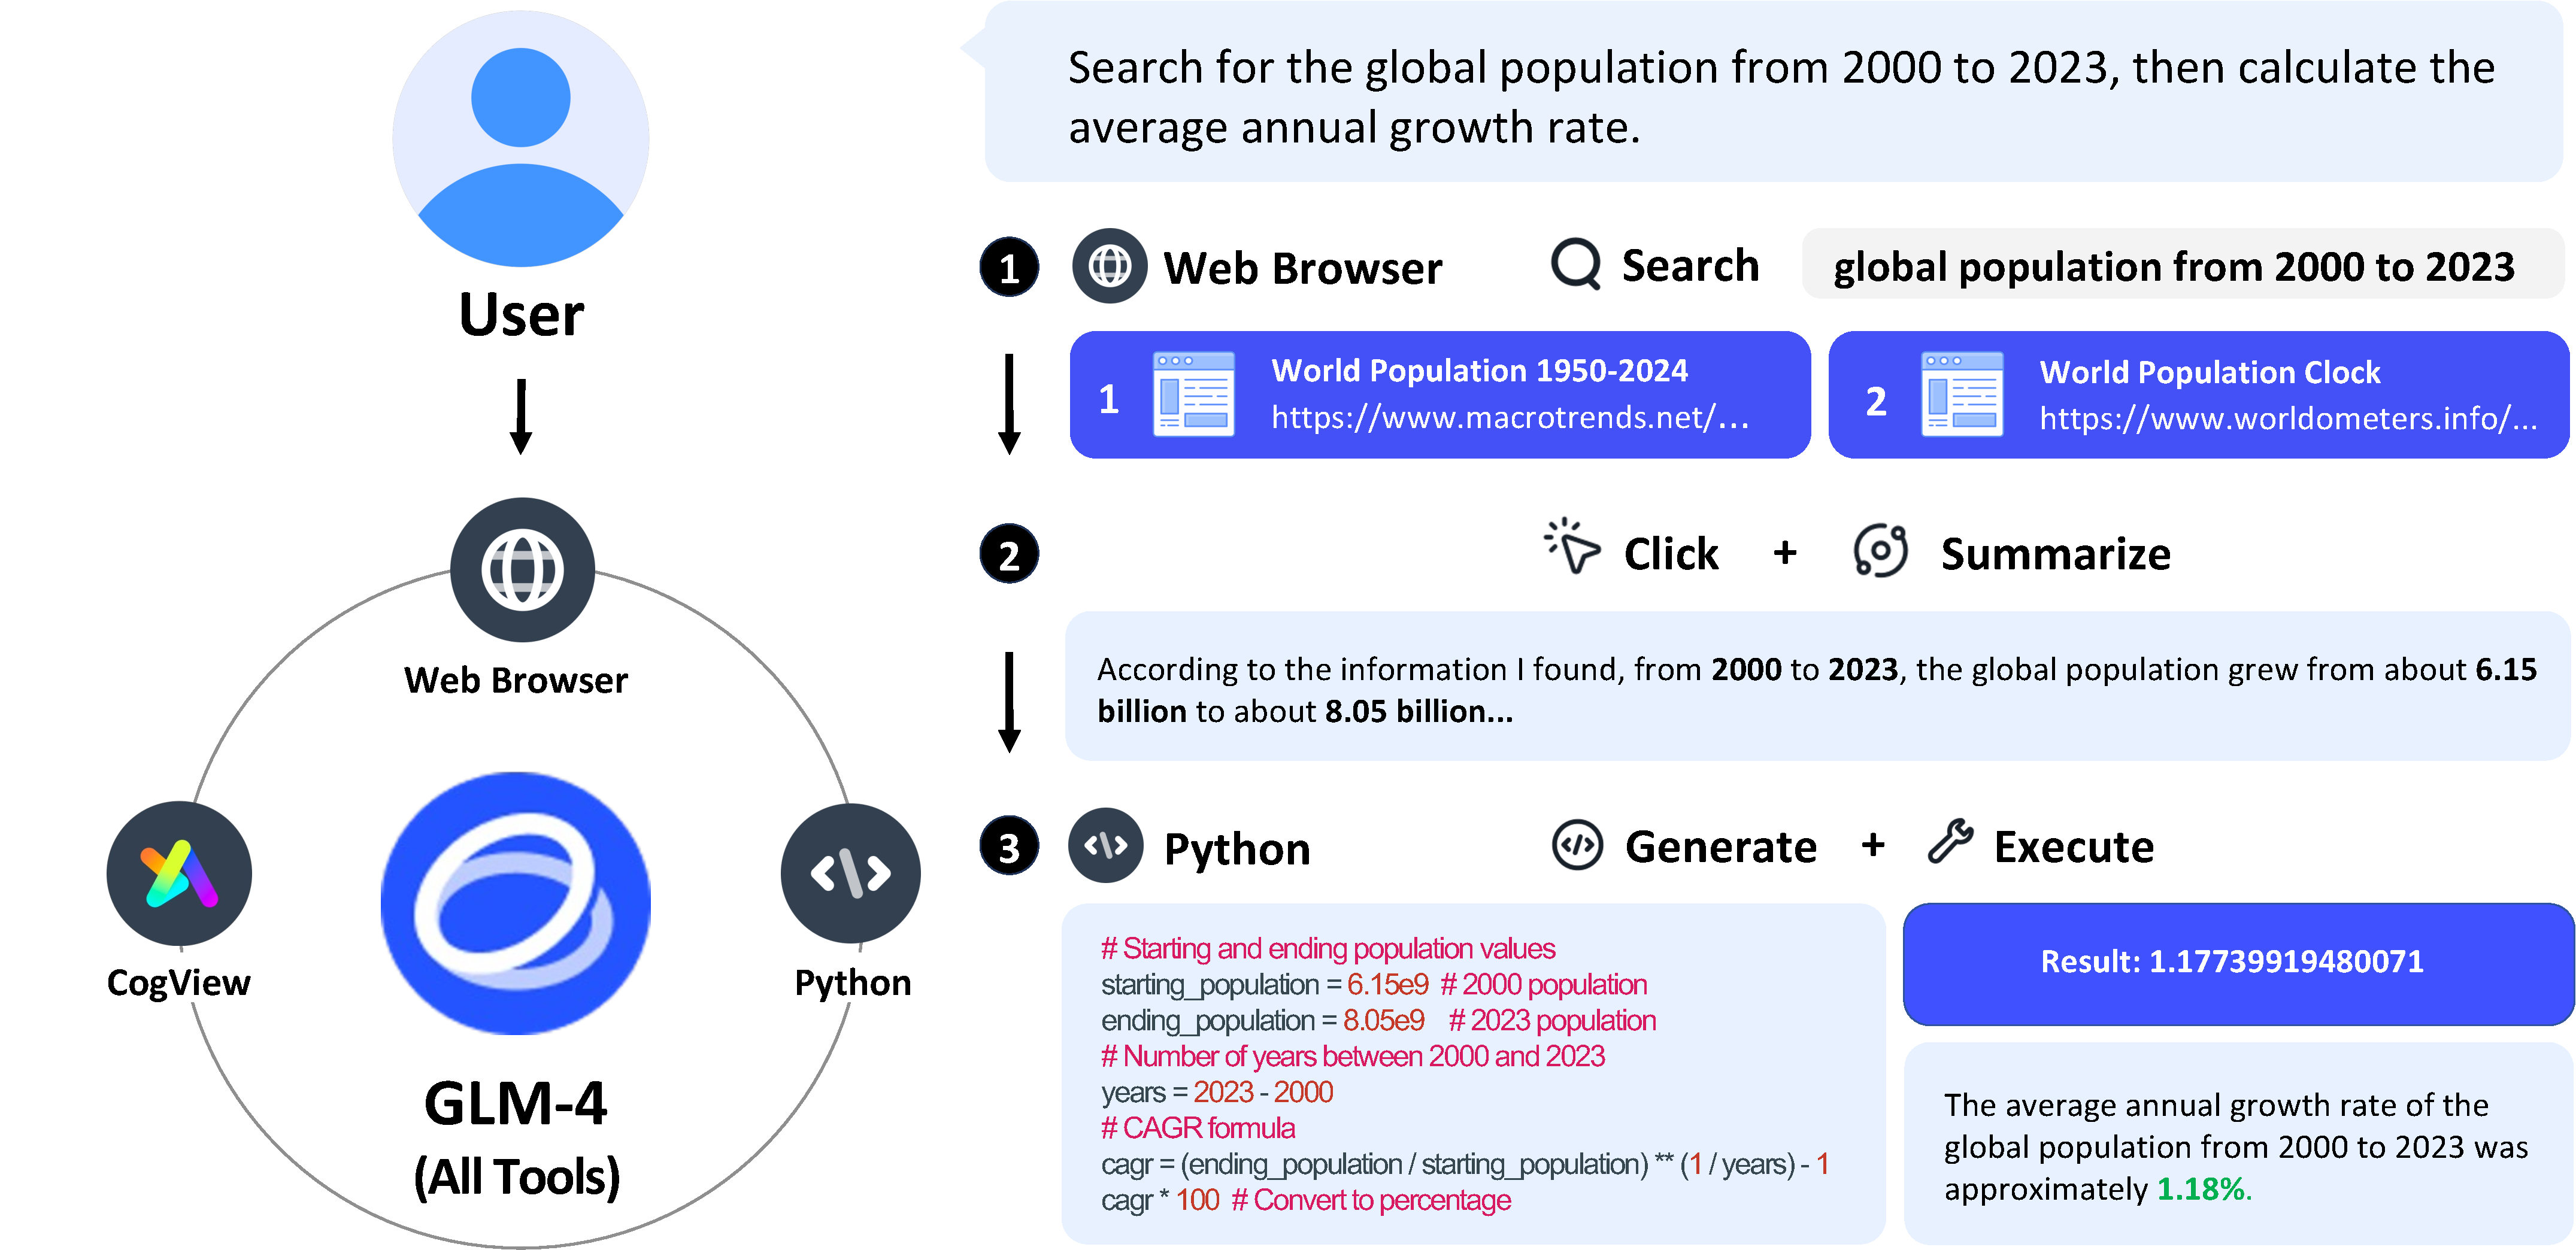
\includegraphics[width=\linewidth]{figs/alltools-example-2.pdf}
    \caption{An Illustrative Example of GLM-4 All Tools.
    }
    \label{fig:alltools-example}
\end{figure}

First, on the most commonly-used English academic benchmarks---MMLU, GSM8K, MATH, BBH, GPQA, and HumanEval, GLM-4 0520 achieves performance closely comparable to that of GPT-4 0613~\cite{openai2023gpt} and Gemini 1.5 Pro~\cite{geminiteam2023gemini}. 
For example, it scores 83.3 vs. 86.4 and 83.7 on MMLU, respectively. 
Second, according to IFEval~\cite{zhou2023instruction}, GLM-4's instruction following capacities on both prompt and instruction levels are approximately as effective as GPT-4-Turbo in both English and Chinese. 
Third, in terms of  Chinese language alignment, GLM-4 outperforms GPT-4 and matches GPT-4-Turbo across eight dimensions in AlignBench~\cite{liu2023alignbench}.   
Finally, for long-context tasks, the GLM-4 (128K) model matches the performance level of GPT-4 Turbo and Claude 3 Opus as measured by LongBench-Chat~\cite{bai2024longalign}, i.e., 87.3 vs. 87.2 and 87.7, respectively. 


\begin{table}[t]
\centering
\renewcommand{\arraystretch}{1.4}
\caption{Performance of Open ChatGLM-6B, ChatGLM2-6B, ChatGLM3-6B, and GLM-4-9B.}
\resizebox{\textwidth}{!}{
\begin{tabular}{@{}ll|rrrr@{}}
\toprule[1.2pt]
Language                  & Dataset          & ChatGLM-6B & ChatGLM2-6B & ChatGLM3-6B-Base & GLM-4-9B \\
                          &                  & \small{(2023-03-14)} &
\small{(2023-06-25)} & \small{(2023-10-27)} & \small{(2024-06-05)} \\
\midrule
\multirow{6}{*}{English} & GSM8K            & 1.5        & 25.9        & 72.3  & 84.0             \\
                          & MATH             & 3.1        & 6.9         & 25.7  & 30.4           \\
                          & BBH              & 0.0        & 29.2        & 66.1    & 76.3         \\
                          & MMLU             & 25.2       & 45.2        & 61.4 & 74.7             \\
                          & GPQA & - & - & 26.8 & 34.3 \\
                          & HumanEval        & 0.0        & 9.8         & 58.5    & 70.1         \\
                          & BoolQ            & 51.8       & 79.0        & 87.9   & 89.6          \\
                          & CommonSenseQA    & 20.5       & 65.4        & 86.5  & 90.7           \\
                          & HellaSwag        & 30.4       & 57.0        & 79.7  & 82.6           \\
                          & PIQA             & 65.7       & 69.6        & 80.1  & 79.1           \\
                          & DROP             & 3.9        & 25.6        & 70.9   & 77.2          \\ 
                          \midrule
\multirow{3}{*}{Chinese} & C-Eval           & 23.7       & 51.7        & 69.0  &     77.1    \\
                          & CMMLU            & 25.3       & 50.0        & 67.5 & 75.1             \\
                          & GAOKAO-Bench     & 26.8       & 46.4        & 67.3 & 74.5            \\
                          & C3               & 35.1       & 58.6        & 73.9  & 77.2         \\
                          \bottomrule[1.2pt]
\end{tabular}
}
\label{tab:6b-performance}
\end{table}

The GLM-4 All Tools model is specifically aligned to better understand user intent and autonomously select the most appropriate tool(s) for task completion. 
For example, it can access online information via a web browser in a multi-round manner, use the Python interpreter to solve math problems, leverage a text-to-image model to generate images, and  call user-defined functions. 
Figure \ref{fig:alltools-example} shows an illustrative example of GLM-4 All Tools with a web browser and Python Interpreter for addressing the user query of ``Search for the global population from 2000 to 2023, then calculate the average annual growth rate''.  
Our first-hand test shows that it not only matches but often surpasses the capabilities of GPT-4 All Tools for common tasks. 





Following our three generations of open ChatGLM-6B models, we also openly released the GLM-4-9B (128K and 1M context length) model. 
GLM-4-9B is pre-trained on approximately ten trillion tokens of multilingual corpus with a context length of 8192 (8K) and post-trained with the same pipeline and data used for GLM-4 (0520). 
With less training compute, it outperforms Llama-3-8B~\cite{llama3} and  supports all the functionality of All Tools in GLM-4. 
We also provide an experimental model GLM-4-9B-Chat-1M with 1 million (1M) context length (about 2 million Chinese characters). 
\Cref{tab:6b-performance} shows the performance of the three generations of ChatGLM-6B models and GLM-4-9B, illustrating the progressive improvements of ChatGLM over time.  


 
\begin{figure}[!ht]
    \centering
    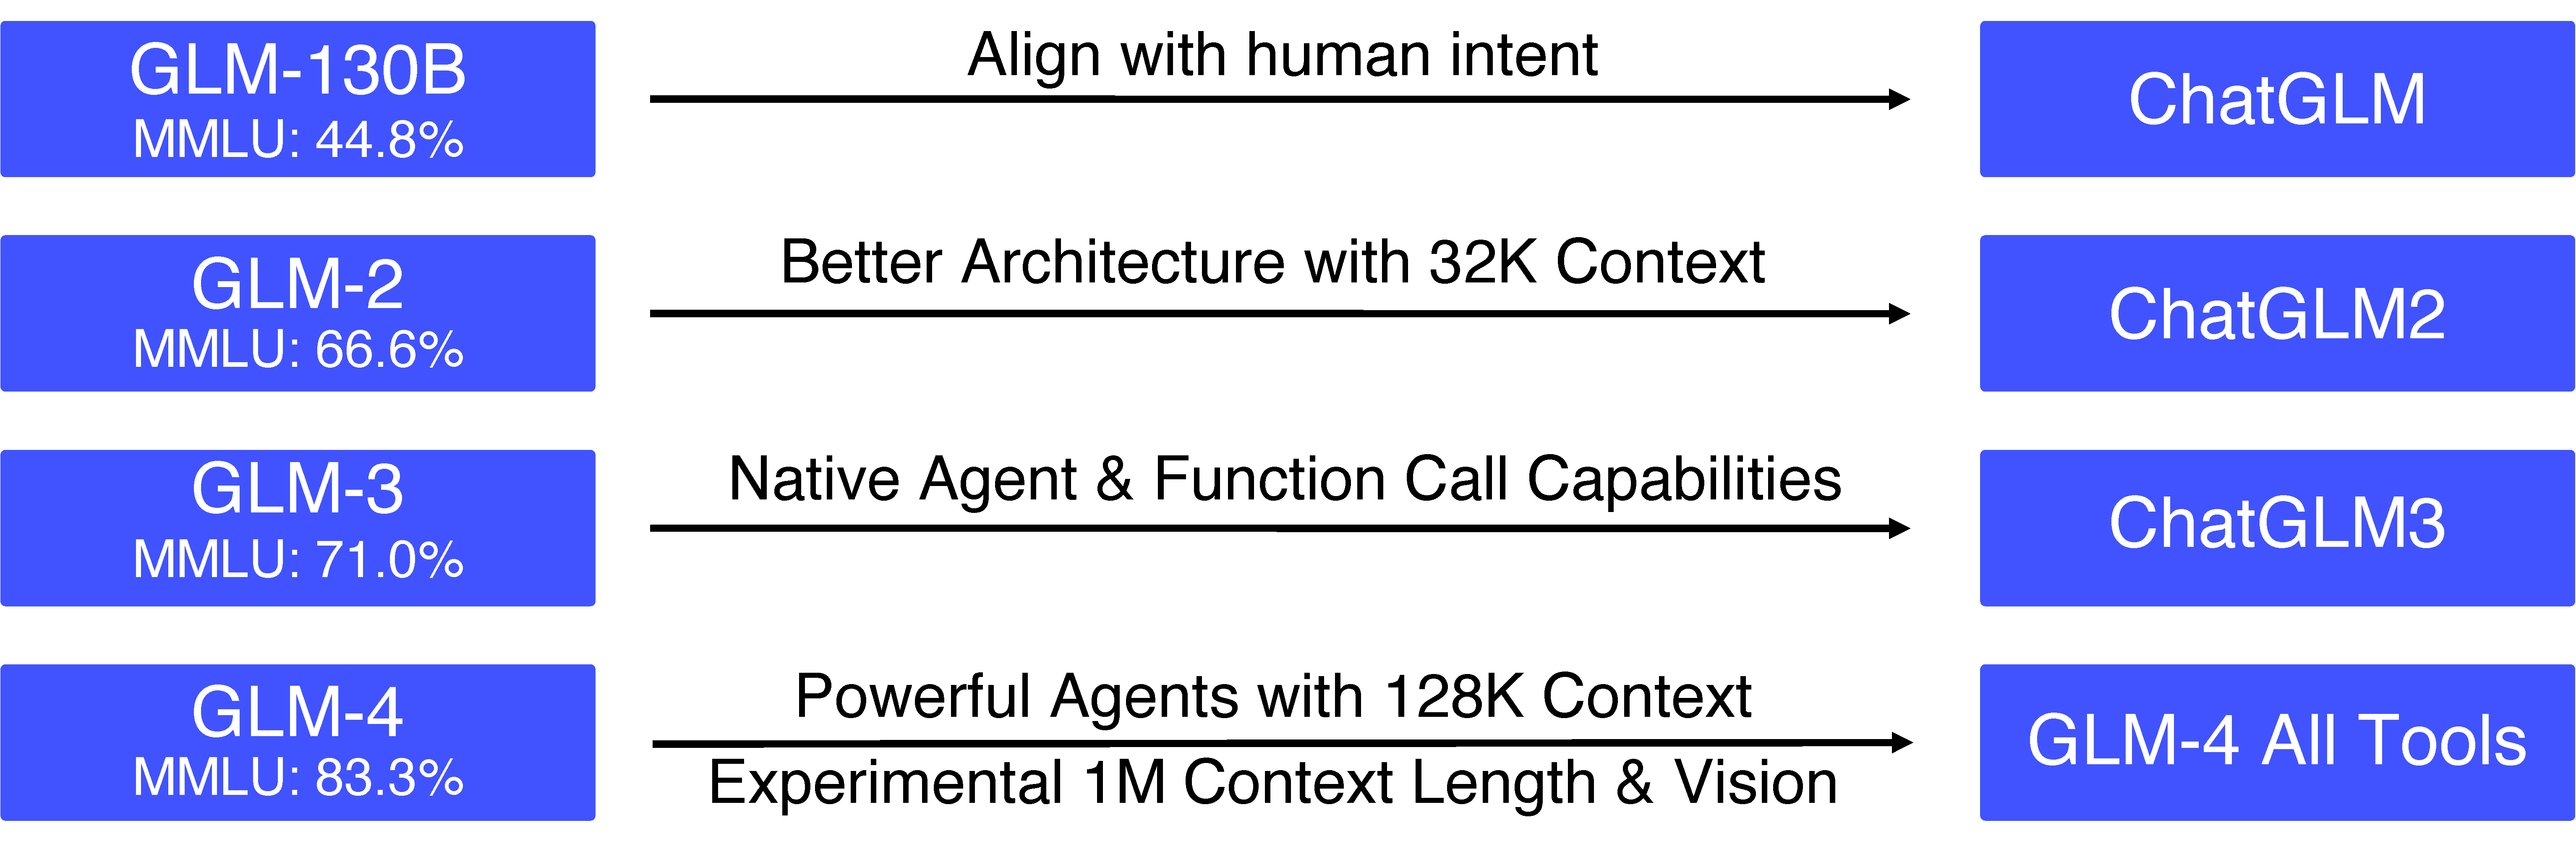
\includegraphics[width=.75\linewidth]{figs/glm130toglm4-2.pdf}
    \caption{From GLM-130B to ChatGLM to ChatGLM2/3 to GLM-4 All Tools. %todo{aohan: Refine this figure}
    }
    \label{fig:glm130-glm4at}
\end{figure}


Figure \ref{fig:glm130-glm4at} summarizes the major improvements and features from GLM-130B to GLM-4 All Tools. 
Throughout this journey, we have also contributed to the open development of the code LLMs (CodeGeeX~\cite{zheng2023codegeex}) as well as visual language models for image understanding (CogVLM~\cite{wang2023cogvlm} and CogAgent~\cite{hong2023cogagent}) and text-to-image generation (CogView~\cite{ding2021cogview,zheng2024cogview3}). 
The open models and data can be accessed via \url{https://github.com/THUDM} and \url{https://huggingface.co/THUDM}. 
 




